\documentclass[11pt]{article}
\usepackage{lipsum}
\usepackage[margin=2.5cm, includefoot, bottom=2cm]{geometry}
\usepackage{fancyhdr}
\usepackage{verbatim}
\usepackage{graphicx}
\usepackage{amsmath}
\usepackage{textcomp}
\usepackage[justification=centering]{caption}
\pagestyle{fancy}
\begin{document}
	\begin{titlepage}
		\begin{center}
			\line(1,0){300}\\
			[0.25in]
			\huge{\bfseries To Create and Compare the Predictive Accuracy of a Genetic Program and an Artificial Neural Network to Predict Corporate Bankruptcy: Final Report}\\
			\line(1,0){300}\\
			[1.5cm]
			
			 \textsc{Carl Saptarshi}\\
			 \textsc{\large  Student Number: 640032165 \\
			 April 2017}
			 
		\end{center}
	\end{titlepage}

\tableofcontents
\thispagestyle{empty}

\cleardoublepage
\setcounter{page}{1}
\section{Background and Introduction }\label{sec:intro}


Due to the dynamic and volatile economy that we live in, the number of companies filing for Corporate Bankruptcy (CB) are rising, especially in times of economic uncertainty, for example, during a period of recession. In turn, being able to predict the likelihood of a corporation going bankrupt and filing for bankruptcy is very important and has been a focal point of issue in accounting research and analysis over the past thirty years \cite{?}.

At present, copious amounts of historical financial data can be extracted from a range of small, medium and large companies. Through looking at some of this data, we can see whether a company has declared bankruptcy or not as yet. Unfortunately, there is not a straightforward way to identify whether a company is \textit{currently} financially distressed and the likelihood of the company going bankrupt in the foreseeable future based on their raw data alone. By selecting appropriate key performance indicators (KPI's) - financial variables that are known to affect a company's performance the most - this data can be manipulated and combined in various ways to help find a way to predict if a company is likely to go bankrupt and if they are financially distressed. The combination of these KPI's should be able to classify any sized company. \\
A \textbf{\textit{genetic program}} (GP) can be used to generate and evolve mathematical expressions to produce an intuitive function that could classify whether a company is financially distressed and likely to go bankrupt. Therefore, the aim of this dissertation is to create a GP which will produce a function that will predict if a company is likely to go bankrupt. This model will then be compared against other benchmark models already made to compare their predictive accuracies. \\

\subsection{Background into Bankruptcy}
\subsubsection{What is Bankruptcy' }\label{sec:bankdef}
When a company (the \textit{debtor}) takes out a loan or borrows money from somewhere like a loan company(the \textit{creditor}) , it is up to the debtor to ensure that the creditor is repaid the full amount that was borrowed subject to the creditors terms and conditions.


If the debtor starts to fall behind on their payments and are unable to repay their debts, the debtor may file for a Chapter 7 bankruptcy in which the court will appoint a trustee to shut down the company and liquidate their assets, for example, by selling machinery, land and company shares to recover some money which they the trustee can give back to the creditor to clear the company's debt. If the company is still unable to pay back the debt even after this, the company will be terminated. As economies have grown rapidly since 1960's, especially in the western part of the world, bankruptcy has been recognised on a much grander scale \cite{?}

\subsubsection{Who does it Affect?}
Bankruptcy does not just affect those that are employed within that company; it also affects third party members such as shareholders, investors, and company clients. CB has been an area of interest, especially in the field of financial analysis and for stakeholders who are interested in the performance of the company \cite{?}. Since the 1960's, empirical risk assessment models have been developed which have been used to predict CB. 

Using financial data of a company, the likelihood of CB can be predicted for \textit{'n'} number of years ahead. 
Loan companies can use this information to determine whether loans should be granted to a corporation, as they will know the likelihood of a company defaulting or not \cite{?}. This has helped to give banks competitive advantages, as they become aware of how likely a company will be to default, and is able to predict customer behaviour in times of difficulty \cite{?}.

Looking at reports from the American Bankruptcy Institute \cite{?} showed that in the year 2000, 35,742 companies filed for bankruptcy, 43,546 companies in 2008 and 60,837 by 2009, at the peak of the recession. By 2012 this fell to 40,075 and 24,114 by 2016 . These statistics clearly indicate the volatility and uncertainty in the economy as it changes, which is part of what makes CB prediction incredibly important.

\subsection{Algorithms for Corporate Bankruptcy Prediction}
As the aim of the project to classify whether a company is likely to go bankrupt, this type of problem can be called a binary classification problem. This takes a series of inputs and returns a classification which determines whether or not a company is financially distressed. Companies likely to suffer from financial distress will have certain characteristics associated with them, similarly for companies not facing this problem. This means that the data being used should be linearly separable when classifying the data, making this a linear binary classification problem. As it is difficult to compare very small companies with very large corporations, to make them comparable, the data used tends to be standardised. This helps to scale the data into units where all companies of any size can be compared. 

 There have been several techniques that have been used to predict CB, some of which will be introduced here.  

\textbf{Individual Ratio Selection (IRS)} -This process involved selecting 30 financial variables, and converting these to ratios. Based on a threshold for each variable, this would determine if a company is financially distressed or not.

\textbf{Multivariate Discriminant Analysis (MDA)} - Altman created this technique in the 1960's, which takes uses a discriminant function to score a company \cite{?}. This function uses five financially weighted ratios. Based on the overall discriminant score, the company can be classified as financially distressed or not.

\textbf{Supervised Learning (SL)} - Some of the current methods to predict CB fall under the umbrella of Machine Learning (ML). ML is a form of Artificial Intelligence that allows a computer program to learn without the use of explicit programming \cite{?}. This means whilst the program is running, it will start to determine patterns in the data, and adapt the program appropriately to try to produce the best predictions and classifications.
In SL, the output after each iteration of each model is compared against the already known desired output. This can then be used for checking the model's classification accuracy. For every iteration, the model will start to learn, so the classification accuracy will start to improve over time. Eventually, when an unknown set of data (hold out data) is inputted into the model, it will be able to correctly produce an output to declare if the company in question will go bankrupt or to a certain degree of accuracy.

\textbf{Genetic Program (GP)} - GPs fall under the umbrella of Evolutionary Computing. Algorithms that belong to the EC family are inspired by biological evolution and used for optimisation problems. A Genetic Algorithm is one such member, inspired by Darwins Theory of Evolution. Genetic Programs are a type of GA which have been used for prediction and classification. A population of functions is created where fitter individuals in the population are more likely to survive and produce offspring that are (in theory) more suited to their environment. The aim of this is to create an optimal function which can give the most accurate classification prediction on unknown data to see if a company is likely to go bankrupt within one year. 

\textbf{Artificial Neural Networks (ANN)} - Also known as the Multi Layer Perceptron (MLP),  this technique is inspired by the interconnectivity of the brain and applies this to prediction and classification \cite{?}. ANN's are made of an input layer, hidden layers and an output layer which produces a classification based on the input. The network uses the weights on its neural that connect each node to the next layer, which are tweaked, based on the accuracy error, to allow the network to learn and give an accurate classification for unknown data. 
\\

In this report, I will be discussing how I developed and compared an ANN and GP to predict CB.  I start by introducing some of the research that was conducted to gain a deeper understanding of what this project entailed. Using this research, I then discuss the requirements that were needed to complete the project. When talking about ANN's, assume that the ANN structure follows the format \textit{(input, Number of nodes per layer, output)} format. Using this research, I then formulate my design specification which was used to form the structure of the models that were implemented to test the predictive accuracy of the two models. After this, I will go on to talk about how the models were tested individually and compared against each other, before giving an evaluation of the project that has been completed. After this, I will then mention work that could be completed in the future to potentially improve this project, before coming to final conclusions. 
%\newpage
\section{Summary of literature review and specification}\label{sec:spec}
\subsection{Literature Review}
All the techniques mentioned in section 1.2 have been used extensively in the area classification and prediction. Altman and Ohlson , pioneers of CB prediction since the 1960's selected financial variables from multiple company's bank statements to predict CB \cite{?}. These variables (\textit{key performance indicators} (KPI's)) were used as they believed these were important factors that indicated a company's performance. To make companies more comparable, both techniques involved converting the KPI's into ratios as a method of standardising the data. Newer models proposed are based around Altman's financial ratios and use their prediction accuracy for MDA and IRS as benchmarks to compare their new proposed work against techniques already in use. 


Beaver introduced the idea of using financial ratios which could be used for CF prediction. Financial ratios were selected one at a time. Using the results of each of the outputs of the ratio values, they would be used to give an overall prediction as to whether or not a company would fail.These ratios would be used in order to get a binary classification as to whether a company is likely to fail or not. For each ratio, a threshold value was set. If the ratio was below the threshold, it failed, otherwise it would not fail.


Altman used MDA in order to approach the task of CB prediction. He took an empirical set of financial variables and created financial ratios which were KPI?s that would be associated with failure prediction. This was essentially a linear model which was used in order to classify between non-failed companies and companies that are likely to fail.MDA allows for multiple ratios to be used as inputs and to be associated with weightings, to provide a classification of a selection of ratios simultaneously, making this very accurate and efficient, producing 95\% predictive accuracy. 

The MDA technique was favoured as used multivariate data at once to get an overall prediction rather than taking each ratio and scoring that to give predictions \cite{?}, making this superior to IRS, but only if the KPI's were jointly distributed according to a multivariate normal distribution \cite{?}. \\
Wilson  \cite{?}and Lensburg \cite{?} used newer approaches by implementing ANN's and GP's respectively to this classification problem. Both of these techniques can handle noisy data that is unevenly distributed better than Altman's MDA, showing that both ANN's and GP's have potential to be more accurate than IRS and MDA. 

ANNs tend to perform very well in terms of performance and accuracy. Wilson et al used an ANN approach with a (5, 10, 2) structure \cite{?}. To improve predictive accuracy, the Monte-Carlo technique was used to give a better representation of classifications. Overall, they achieved a 97.5\% accuracy on their testing dataset, making this much more accurate than MDA and IRS. \\
Lee used a decision tree (DT) method to predict CB \cite{?}. Lee used 8 different KPI's when approaching this problem. Using this GP model, the testing accuracy of 92.91\%. Rostamy \cite{?} used a similar approach to Lee, using five different KPI's. After training the GP, it could correctly predict if a company would go bankrupt or not 90\% of the time, which was like MDA, however more flexible in terms of the type of data that could be used.

GP's may work slower as they explore a large search space and may be restricted to certain limitations e.g. a maximum tree depth. For each crossover and mutation, the depth of tree may increase. This can increase the computation time rapidly. When designing and implementing the GP, these factors will typically be accounted for as seen in Etemadi's et al paper \cite{?}. \\

Through the research completed, many papers used Altman's KPI's as their inputs. However, as Altman suggested, these ratios may not necessarily be the most optimal, but these still provided the best alternative discriminant function to work with at the time \cite{?}. Since then, economies have changed significantly, these ratios may not necessarily be the best to use to predict CB, but may still be significant enough to give an accurate enough prediction. As seen by Back, Rostamy and Lee\cite{'''}, other ratios have been used to predict CB, and achieved similar results to MDA, which could potentially be more significant now. Wilson used Altman's KPI's and achieved the 97.5\% accuracy, with far fewer ratios relative to Back and Lee, which must be taken into consideration \cite{?}.
\subsection{Project Specification}
After careful consideration of the researched techniques, I will be predicting CB using ANNs and GPs due to their strong predictive accuracy rates and ability to handle noisy data. Though they do have drawbacks, I will aim to minimise these through the project specification and implementation.\\

As the models used in the research depended on various datasets, the first thing that needed to be acquired was a dataset with an enough data, and containing enough variables that could give an indication as to whether a company went bankrupt or not. The decision to use only small to medium enterprises(SME) was to have more consistent, comparable data, as shown by Altman. Using this dataset, I would then able to create financial ratios which can then be used in the models to be developed. 

Two programs were intended to be made for this project; a feed forward ANN with back propagation and secondly a regression tree GP.  I have chosen to take forward these two models is that ANNs are known to produce very accurate results efficiently. The reason a regression tree GP has been put forward is because this a valid technique that can be used as they are able to produce a function that will directly map the input KPI's to give a classification.

Both techniques should give an indication as to which KPI's affect the classification prediction, and give an indication as to which KPI's affect the companies and could be a cause of their failure.  \\
As this is a binary classification problem, the output of each model determines whether a company can be classified as likely to go bankrupt or not. To represent the classification,  0 will represent a company that is not likely to go bankrupt  and 1 will represent a financially distressed company.

Since this representation is a number, the actual floating point value of the output (which will be between 0 and 1) for the NN, this number will be used to represent the likelihood of failure as a probability. For example, if the value was 0.618, it could be said that the company has a probability of 0.312 of staying afloat for the forthcoming year. Whereas if the value was 0.111 then the company has a 0.899 probability of staying afloat for the forthcoming year. Here, a clear differentiation can be made between two companies, one which is more likely to fail than the other.
Once the development part of the project is complete, I planned to test the results of both models, individually against each other to compare their predictive accuracies, and against Altman's benchmarks results.

To allow the ANN to learn, I will be using the training dataset. When testing this, I will use a testing dataset to validate the results to see the true accuracy. I will also use K-Fold Cross-Validation techniques to help improve the comparability and the accuracy as well.. To increase comparability, I will also use the same datasets for both ANN and GP.

I will also consider the number of iterations that have been used to complete the task in both ANN and GP. The time it takes to process the inputs will also be compared. To determine what KPI's have a greater contribution than others, for the variables that are being used for ANN's, I will remove one ratio, rerun the programs under the same training and testing conditions to then check the outputted value to see how significantly different the output is with and without that ratio. This will help to determine what ratios have a greater weighting and could be a significant factor in the future success or demise of a company. 

Overall, to make my project successful, I will take these factors into account before starting to program, to prevent any long-term errors that could occur. I will also use a reliable GUI to help prevent programming errors, which in turn will make my project more successful. 
%\newpage
\section{Model Design}
This project follows the Software Development Life Cycle(SDLC) methodology, but more specifically I following the Waterfall Development methodology, except for the literature review. The reason this was chosen is to give a simple, clear structure to the way that I planned on completing the project. As the project had been planned through the research undertaken, it was now possible to move onto the design of the models. 
\subsection{Data Collection}
Firstly, I had to collect all the data that I planned to use. The data that collected had been given to me by the University of Exeter Business School as they had access to multiple years' worth of data for several companies. As each economy is different, companies may perform better or worse in different economies, therefore to make the data more comparable, the data that collected was solely from American companies from the US economy.

The dataset collected contained 671 rows of data, with 31 different variables. Out of these, only 8 of were financial variables KPI's. For example, \textit{net income} and \textit{sales} would be KPI's that could affect the company performance, however variables like \textit{company name} and \textit{ticket}, would be much less likely to affect the company's performance. Therefore, to make the data more usable, variables not considered to be KPI's were removed from the dataset. Any rows with incomplete data were also removed. These were rows of data in which a cell contained a question mark in any of the cells for a company. Now the dataset contained only complete data with the key financial variables. Due to the types of the companies being given, to make smaller companies comparable to larger companies, the KPI's were standardised into five ratios, like the methods that Altman used to standardise his dataset. This new standardised dataset contained five KPI ratios and their associated classification, labelled \textbf{X1,..., X5}, each representing a specific ratio:
\begin{center}
	\begin{minipage}{.6\textwidth}
		\begin{itemize}
			\item[] \textbf{X1} - working capital / Total Assets
			\item[] \textbf{X2} - Retained Earnings / Total Assets
			\item[] \textbf{X3} - Earnings Before Interest and Tax / total Assets
			\item[] \textbf{X4} - Market Value of Equity / Total Debt
			\item[] \textbf{X5} - Sales / Total Assets
			\item[] \textbf{Failed} - 0 or 1
		\end{itemize}
	\end{minipage}
\end{center}
For an explanation about these KPI's and why these ratios were chosen, please refer to Appendix \cite{?}.
Since this dataset was now in the right format, the next stage was to design the ANN and GP that were to be implemented. 
\subsection{Artificial Neural Network Design}
\begin{figure}[h]
\centering
\captionsetup{justification=centering}
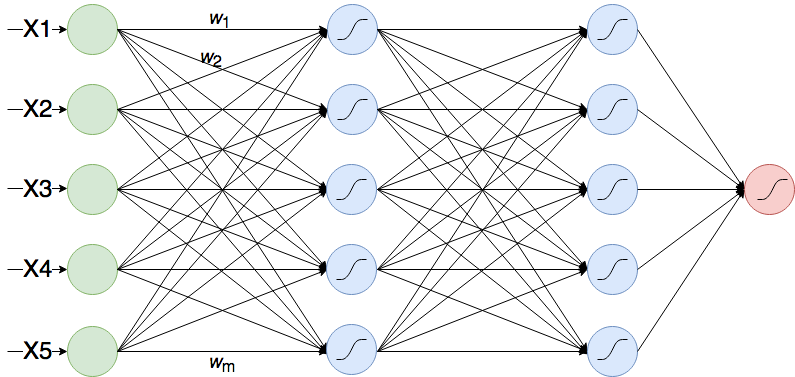
\includegraphics[scale = .37]{ANN}
\caption{Structure of an Artificial Neural Network. Green nodes indicate the input features. Blue nodes indicate hidden nodes and hidden layers, with a sigmoidal activation function. Red nodes indicate the response vector (the output) with a sigmoid function } 
\end{figure}
I chose to implement a feed forward artificial neural network, based on the research conducted in section 2.1. The papers that implemented an ANN used a feed forward network for this binary classification problem, which based on their results, proved to be more than adequate in the area of prediction with only two possible outputs.\\
A feed-forward ANN usually follows the same layout which makes them applicable to an array of complex problem. The basic structure of the ANN can be seen in figure1, which consists of an input layer, hidden layer(s) and an output layer. The input layer consists of the feature vector which represents the data inputs as a single layer of nodes. The hidden layer(s) and hidden nodes are used to help reduce alter the representation of the data by transforming it, and reducing any non-linearity's in the data. The output is a response vector that can consist of a single node, which will output the feature vectors classification. Connecting the nodes in each layer is accomplished using weighted neural synapses, that connect each node in the current layer to each node in the next layer. Since ANNs have been used multiple times for this particular type of binary classification problem, the ANN designed to be a benchmark for predictive accuracy on this particular dataset, which can be compared against the GP that will be developed. 

\subsubsection{Input Layer and Synaptic Weights}
Since ANN's can cope with high dimensional, non-linear data, I initially decided to use all five of the KPI ratios as the input feature vector that was created from the dataset as the ANN would be more than capable to handle all this data at once.\\

Due to the stochastic nature of an ANN, when initialising the network before the data from the input features are read into the network, the weights that each node in the previous layer to each node in the next layer also needed to be initialised. As part of the design, I chose to completely randomise the weights on each of the synapses. If the weights were not initialised randomly, when the network starts to learn, it would learn in the exactly same way every time the program is run because the network will always start at the same position in the search space, which means it will always follow the same route to get to a solution which would always be the same since the stochastic element has been removed.  By initialising the weights randomly, the symmetry of the network is broken, which allows the network to be initialised differently, so the weighted input signal that moves from one layer to the next would always be different, allowing more of the search space to be explored, which would allow more solutions ( possibly more optimal solutions ) to be found.
\subsubsection{Hidden Layers and Activation Function }
The next step in ANN design is the structure of the hidden layers of the network.  Figure 1 shows an example of an ANN with a (2,5,5,1) structure. Through research, it was found that when using one hidden layer with multiple nodes, the network is more likely to start memorising the data being passed to it, which can cause the network overfitting. This means that when testing the predictive accuracy of the hold out data, the worse it will generalise, and give a poor predictive accuracy. Therefore, to avoid this, I will use multiple hidden layers as this would allow the network to generalise better without network memorisation.  To make it easier for the user to input their own ANN structure, I will provide a configuration file for custom ANN configuration file. 

Each neurone in the hidden layer transforms the values from the previous layer with a weighted linear summation.The cumulative sum of these products (\textit{z}) is used as input to the next node in the hidden layer, which then is passed through a nonlinear activation function. For the ANN that is being designed, I will initially use a sigmoid activation function, as indicated by the sigmoidal curves in each of the hidden nodes in Figure 1 and equation 1. \begin{equation} sig(z) = 1/1+e^{-z} \end{equation}
The sigmoid function adds an element of non-linearity to the to the model, which allows the computation of nontrivial problems using only a small number of nodes, which is what makes this function much more popular relative to other activation functions like a step function.
\subsubsection{Output Layer and Learning Mechanism}
The output layer receives the values from the last hidden layer and transforms them into output values. When training the network, I will classify the outputs as either a 0 or 1 by passing the raw value through another sigmoid activation function. To begin with, if the value outputted is below 0.5, then it will be classified as a 0, otherwise it would be classified as a 1. Using this, the error percentage can then be measured against the true results, and the weights will be altered accordingly using a learning mechanism. For this network, the back - propagation learning method should be sufficient enough to allow the network to learn, and try to minimise the error rate by manipulating the weights on the synapses, to give the best possible accuracy, showing that the network has trained.\\
\subsection{Genetic Program Design}
\begin{figure}[h]
\centering
\includegraphics[scale = .39]{GPFlow3}
\caption{Flow chart to represent the Genetic Program that has been designed. Green boxes indicate population generation. Red boxes are the termination criteria and testing. Purple boxes are selection methods. Orange Boxes relate to genetic crossover. Yellow boxes relate to genetic Mutation. Blue boxes related to the fitness function. } 
\end{figure}
The aim of this model is to be able to produce an optimal function that is readable and can predict to a degree of accuracy, whether a company is likely to go bankrupt or not within one year, based on their input data. As this type of model is know to be able to handle noisy and non-linear data, I decided to use all the 5 KPI ratios for my inputs, as these were going to also be the same inputs for the ANN. This allowed for data consistency and made the models more comparable in the testing phase. Through the research conducted, I was now able to start formulating the design for the GP.  Figure 2 shows the entire overview for this design stage. Each colour represents the main stages that were required to allow the GP to be successful in design and implementation with the aim of producing an optimal function.  The main stages of the GP include generating a population (green boxes), finding a fitness function(blue boxes), selecting parents (purple boxes), crossing over and mutation of parents to produce children (orange and yellow boxes respectively), and finally the termination criteria (red boxes). 
\subsubsection{Data Representation}
Through out this project, each member of the population will have to have some form of representation. Here I will mention some of the ways that the data could be represented which I planned to implement in section 4. 

An example of a random population generated containing 4 members can be seen below. Each member is represented as a string, using standard infix notation and the entire population is stored within a list. Infix notation is a format expressions tend to be written in, where 2 operands surround an operator. The reason for this is because when an optimal function is found, it will be returned as a mathematical function, which are typically represented in this particular format. 
\begin{align*}
pop_n = [``X1+1.3-X3+X2/X4*X5" ,``X2/X5+(6.433-X1)*X3*X4", \\
``X1*9.56-(X2*(X5*X4))-X3", ``4+8.22/X1*X2-7+X3/X4*X5"] 
\end{align*}
To make the crossover and mutation process simpler, I decided to represent the parent genotypes using the lazy instantiation of a \textit{binary expression tree} data structure. Lazy instantiation is the process of performing an action only when required. Binary trees are easy to understand, implement, and make the process of genetic crossover and mutation significantly easier as the model learns. The reason I chose lazy instantiation was because it would save computation time from having to generate binary trees for every single member of the population, even though only the two selected parents will be going through the genetic operators to create children. Below is an example of a two expressions converted into binary trees. 
\begin{figure}[h]
\centering
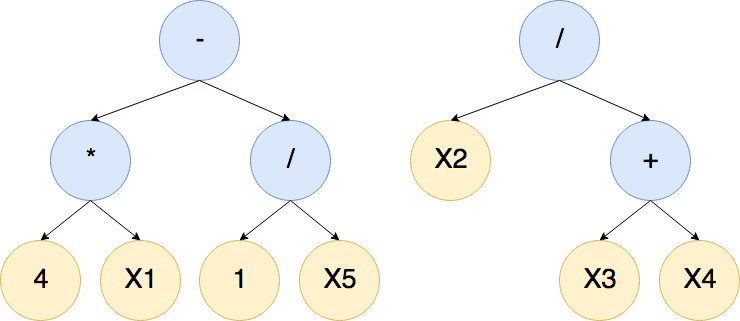
\includegraphics[scale = .30]{binaryT}
\caption{Infix expressions: ``4*X1-1/X5" and ``X2/(X3+X4)" converted into binary trees. Operators represented as blue nodes. Operands represented as yellow nodes. } 
\end{figure}
After the processes of genetic crossover and mutation are completed, the children need to be put back into the population if they are fitter than the worst members in the population. Therefore since the children have to be in the infix format, the binary trees have to be parsed back into an infix notation which the population will accept. 
\subsubsection{Generating a Population}
It is very common practise to initialise a population randomly in GPs. The reason for this is to allow different populations to begin in different areas of the search space, such that they can explore different areas to try to find the global optimum solution, which in this case would be the best predictive accuracy.  This population would consist of randomly created mathematical functions, each of which representing one member of the population. A mathematical function consists of two parts; the functional set of operators (+,-,*,/) and terminal set of operands (numerical values and variables X1,...,X5). To create an random individual, I decided to design a mathematical expression generator. This would allow random, valid functions to be created using randomly selected members of the functional and terminal sets and would represent an individual's genotype. To begin with, a population would consist of 500 randomly generated individuals. Based on the arities of the functional operators, the randomly generated population was based on the \textit{full} method of population generation \cite{?} rather than \textit{grow} or \textit{ramped half \& half} \cite{?}. Based on the arities of the functional set, the full method provided sufficient variety in expression generation.
\subsubsection{Fitness Function}
The next step is to evaluate the fitness's of the individual expressions in the population. This would represent the phenotype of an individual, i.e. how good the individual is suited to its environment, representing how close it is to an optimal solution. This can be done is through calculating the error between the true classifications of the data set and the predicted output as given by the function. The aim of this is to minimise the error between the actual classifications and the number of incorrectly predicted classifications produced by the function where the optimal function which correctly classified every company would have a fitness value of 0. This can be called a minimisation problem where the objective is to minimise the fitness function. \\
For this I will use the \textit{Number of Hits fitness function} \cite{?} . This fitness function is calculated by firstly passing each row of data through the function. For each row of data, the output will either be a positive or negative number given by this function. If the value is greater than 0, it is classified as 1, otherwise 0. Using these classifications for each predicted row of data, these can now be compared against each of the true classifications from the data. For every row of data that is classified correctly, the fitness value does not increase. However for every misclassification, the fitness value for that function increases by 1. This shows that a good function which has more number of hits would have a lower fitness value, and a function which has a high misclassification rate has a high fitness value. 
\subsubsection{Selection}
For most GPs, genetic operators such as crossover and mutation are applied to certain individuals in the population based on their fitness value. The better the individual is in the population, the more likely they are to produce children functions. Therefore,
to select these parents, I have chosen to use \textit{tournament selection} \cite{?}. This works by selecting a random subset of the population, \textit{t}, and then comparing the fitness's of each of members of \textit{t}. The individual with the best fitness value i.e. closest fitness to 0, will be selected to be the first parent. This same process will occur to select the second parent. An individual can only be selected once per generation, as the same member of the population cannot be selected to be both parents. This will keep the selection pressure relatively constant as it does not necessarily favour the best individuals in the population, rather it selects the best individuals in the random subset of the population selected as candidate parents. 
\subsubsection{Genetic Operations}
Using the parents, the children can be created using the genetic operators - \textit{crossover} and \textit{mutation}. Typically, in a GP, crossover occurs first. I decided to use a single subtree crossover between the parents, which create two children, each containing parts of both parents. This should be relatively easy since the parents will be in the expression binary tree format. 
After the two new children have been created, the genetic operator,  \textit{mutation} can be used on the children. This is used to help maintain genetic diversity within the population from current generation to the next.  Here, I will be using \textit{single point mutation}, where a random node on each of the parents will be selected and be altered based on its arity. For example, if the node selected is a numerical value, with an arity of 1, then this will be replaced by another value with an arity of 1, and similarly if the node selected has an arity of 2, then it will be replaced by another functional node.
\subsubsection{Termination Criteria}
The termination criteria will be checked in multiple places. The first termination criteria is if an optimal function has been found in the population. Since there is a possibility of this occurring when the population is evaluated, this should be checked before the program GP continues. If an optimal solution does exist, then return the best individual. If after \textit{n} generations of running the program, if the best individual in the population still has not been able to meet the optimal fitness criteria, then the GP should stop and return the fittest individual in the current population as will have a fitness value closer to 0 compare to all others in the population. 

Using optimal function, it should be tested on the holdout dataset to check the predictive accuracy of the function to see if it has predicted whether a company is likely go bankrupt correctly. This output will then be passed through the same sigmoidal function (eq. 1). Using a 0.5 threshold for the sigmoid function, if the value outputted from this function is greater than 0.499, it will be classified as 1, otherwise 0. This can then be used to give the classification predictive accuracy of the function. 
\subsection{Testing Design}
After the development is completed, various tests could be conducted on both the ANN and GP to see if these tests would alter the learning process and predictive accuracy which will be mentioned now and in the testing phase of the dissertation. The design of the tests has been based on the project specification and on the way the models have been developed. 
The first type of testing I will do is manual testing for the ANN and GP. This will be running  the models' multiple times with smaller datasets with already accepted solutions. This will be able to check whether the models are working and performing as they should be. 
During the development of the program, I will use software testing to determine whether the functions that are being made are functioning in the correct way. After this, I can then perform validation testing by running the model's multiple times to ensure that they are both learning the way they should be, to get to an optimal result .To do this, I will use the \textit{unit} testing , and \textit{black-box} testing to determine whether each function performs the way it should by comparing the desired output of the function to the actual output of the function, and check whether they match. After this, performance testing will be completed on both models, to ensure that they are learning and predicting at an acceptable rate. This will be completed by testing the performance of each function and the overall model to identify the areas of the model which may perform unusually slow. Finally, after the development and testing has completed, I will perform \textit{user acceptance} testing to ensure that the program works and could be used as a product that could be deployed in the future. 
\subsection{Programming Language and Environment}
The final part of the design stage was to determine what programming language and programming environment that could be used for this project. Through careful consideration, I decided to choose Python as my main programming language. The main reasons for this were that since the ANN was going to be used as a benchmark, rather than trying to implement an ANN from scratch, I chose to use a library - \textit{sklearn}, as this provided all the functionality to allow a feed forward ANN with back propagation to be created, along with many other functions which could be used to test the network e.g. using other transfer functions, methods of splitting the data and how to train and test the network. Since Python was what I was going to use for the ANN, for consistency, I also decided to use Python as the choice of language for the regression tree GP. This was because of the fact that Python offers object orientation, speed, high level abstraction for memory allocation and offered others optimised mathematical libraries such as Numpy which can make data handing easier, and Matplotlib which offers easy to make graphs which can then be used for data analysis. 
%\newpage
\section{Development}
To make the development more manageable, I developed the models by attempting smaller problems, with static data. This way, debugging and understanding the errors would be easier. To make the testing of the models more reliable, I decided to use the same dataset for the ANN and the GP. 

Since the dataset was the same for both model, I used the same method to read and split the data sets from their associated classifications. As this was a SL problem, the decision to split the data was because the classifications from the dataset could be used to form the fitness functions for both techniques that were implemented.
\subsection{Development of the Artificial Neural Network}
As the ANN being implemented was going to be used as a benchmark to test against the Genetic Program, rather than implementing the ANN from scratch, as part of the design stage, I chose to use a library in Python - Sklearn, a well-known machine learning library that has the facilities to develop a feed forward ANN quickly, and the ability to train, test, and present the outputs of the data in a variety of ways.  
subsubsection{Multi Layer Perceptron Classifier}
After the data set had been read in, the data was stored in a variable \textit{data\textunderscore CBD} and the classification labels were stored in a \textit{class\textunderscore labels\textunderscore CBD} variable. Since the data was read in using the numpy module, the data was kept in an numpy array, therefore to keep the data and classification labels types the same, I converted this list to a numpy array as well to avoid conflict later. 

As the data was now in the correct format, the ANN could now be implemented. To do this, using the \textit{sklearn.neural\textunderscore network} module, I imported the \textit{MLPClassifer}. Using the MLPClassifier constructor, I chose to use the \textit{logistic} function as the activation function. This is the most population activation to use on feed forward ANNs and part of the project design.

When creating the network, the weights on the synapses of the network are initialised randomly when the model is created by default, therefore this did not have to be accounted for.
To allow the synaptic weights to learn, there were different learning methods available that could be used to train the network. This was the solver parameter.  Since the back-propagation learning method was unavailable, I chose to use the stochastic gradient descent (SGD) as my method of adapting the weights to train the network. This is another learning method used to minimise the error in the network to optimise the classification accuracy on the training data. I chose to have use the L2 regularisation parameter (the alpha parameter). A regularisation parameter is used to penalise networks that are more complex, as they can train networks more accurate, but have tendency to over-fit the data, which means they will have poor regularisation, and poor classification predictive accuracy. 

Another parameter that was used was the momentum parameter. In the process of SGD, the aim is to try to minimise the error function with the intention of trying to reach a global minimum in this case. This is because the aim is to try to minimise the error to get the best possible predictive accuracy. Due to the nature of the data, there is a strong likelihood that the data will get trapped in a local minimum and assume that this solution is the best, when in fact, there may be several better alternatives. Momentum is used with the intension of increasing the size of the steps taken towards the minimum by trying to 'escape' from a local minimum. However, this parameter is invalidated when using any other form of solver other than SGD as momentum is only used in SGD as it minimises gradients. The final parameter used for the MLPClassifier constructor was the \textit{hidden\textunderscore layer\textunderscore sizes}. Based on the research conducted and as part of the design stage, I initially chose to use two hidden layer with five nodes within this layer. 

As this entire network could run the ANN very quickly, I was able to run the neural network against my current dataset and get a result. Now that the ANN had been created, and could be used as a benchmark, I was able to start the development of the genetic program.

\subsection{Developing the Genetic Program}

To being with, a subset of the dataset was used. Whilst develop this model, I started by working on smaller problems using this smaller dataset with inputs and outputs I knew would work, as well as an optimal function which the smaller model could find. The reason this was done is so that whilst developing the smaller program, the structure would be developed correctly, and debugging functions through the development phase would be much easier. 

Once all the functions were created, I could then read in the full dataset to see if an optimal function could be found from the GP. 
 \subsubsection{Generating and Handling the Population}
The first stage in the development process was to create a population of functions based on a the functional and terminal sets, and population size. To do this, I created a class called GenMember.
 The purpose of this class was to handle the current population by generating all the members, finding their fitness's, selecting the parents and updating the population.\\
The first function that was created, \textit{generate\textunderscore expression }was used to generate random mathematical functions in infix notation using recursion. 
The reason recursion was used here is because this was an easy way to create the structure of a subexpression, and the combinations of these subexpressions were used to make an individual function.  
As the size of the expression increases, the longer it will take to evaluate and manipulate the functions,  therefore to ensure that that the expression stays a reasonable length, a \textit{max\textunderscore depth} parameter was imposed when generating the functions.
The output of this are mathematically valid functions with bracketing included. 
Using the project design for the population generation, I used the full method of expression generation to provide sufficient variety in the size of each of the functions produced, based on the maximum depth set. This allowed the functions made to be more organic. 
Unfortunately, since not these functions contain all 5 KPI ratios, I created another function called \textit{get\textunderscore valid\textunderscore expressions}. This function was created with a user defined population size, whilst ensuring that invalid functions were filtered out and replaced with valid functions. 
 \\
The next step was to create a fitness function to evaluate each of the members of the population.
The \textit{get\textunderscore fitness} function is called in two scenarios - when the population is initially created and when a new child is produced. When the population is initially generated, all the individuals need to be evaluated to find the fitness's of all the solutions as an optimal expression may exist within the original population. To evaluate each member, each row of the sample data is fed into the population of expressions, and the total was found. A negative value was classified as 0, otherwise 1. Using this, the actual classification labels from the dataset were then compared to the predicted classification labels. For every incorrect prediction, the fitness error value would increase by 1. Very poor solutions would have a very high fitness value, whereas very good individuals with strong predictive accuracy had a very low fitness value as the aim is to minimise the error, therefore they had a high predictive accuracy.\\

Using the evaluated population, the parents needed to be selected. To accomplish this, I made the \textit{tournament\textunderscore selection} function. The output of this function would be the two individuals selected to produce children through crossover and mutation. 
The population and their associated fitnesses were inputted, as well as a user defined tournament selection size. The size refers to the number of candidates that would be selected from the population, as potential parents. The two individuals that were the best from each tournament would then be the parents. The population and their associated fitnesses were zipped together to prevent a member obtaining the wrong fitness value associated with it. Based on the \textit{selection\textunderscore size} selected, \textit{'c'} candidates were selected randomly from within the population. As two parents are needed for the process of cross over to occur, two tournaments were completed to select both parents.
\subsubsection{Infix to Prefix Conversion}
\begin{equation}parents = [('X1+1.3-X3+X2/X4*X5',170),( 'X2/X5+6.433-X1*X3*X4',243)] \end{equation} \begin{equation}parents = [(['+', 'X1', '-', '1.3', '+', 'X3', '/', 'X2', '*', 'X4', 'X5'], 170),([...],243)] \end{equation}
The parents could now be put into a binary tree structure. To do this, I first converted the infix expressions into prefix expressions (also known as \textit{Polish} notation). This format is easier for the machine to parse into a tree structure.  For this, I used a class called \textit{ToPrefixParser}. Each parent was split into their individual elements along with the string 'stop'. This allowed the conversion from infix to prefix to never go beyond the number of elements in each of the parent lists. To ensure that each component of the parent was split correctly, I used regular expressions to split the strings. 

Since the parents were split correctly, they could now be converted into prefix notation (eq. 3). Using [insert website name here], I manipulated a subset of their functions to convert the infix notation into prefix notation as this website was not enough by itself. The \textit{get\textunderscore operation}  function is used to compare the \textit{0th} element of the expression that is being passed in to the \textit{expected character} that the parser is looking for. If they matched, then the value was popped out of the original expression. The \textit{expected character}was checked throughout the other parsing functions. The \textit{is\textunderscore number} function is used to return a number which is a leaf value. 
However, if the character being checked is a "(" and the expected character is also a "(", then this will call the \textit{get\textunderscore expression} function which in turn would be used to get the subexpression that exists within the pair of parentheses. When  \textit{get\textunderscore expression} is called,  a chain of other functions is called sequentially, which will put the infix notation into prefix notation.
\textit{get\textunderscore expression} calls the \textit{get\textunderscore product} function, which then calls the \textit{is\textunderscore number} function which checks to see if the current character being checked is a "(", in which case the sub-expression is then evaluated, otherwise a number is added to the prefix notation output.  As each character in the infix notation is checked, these functions are called to correctly convert the infix notation into prefix notation. \\ 
After both parents have been converted from infix to prefix notation, the newly converted parents are returned by the \textit{get\textunderscore prefix\textunderscore notation} function.  
\subsubsection{The Node Object}
Now the binary tree was ready to be built. A binary tree consists of two types of nodes; branch nodes and leaf nodes. Branch nodes can hold a value, and have "left" and "right" child references. Leaf nodes on the other hand can hold a value but have no child references. Both branch and leaf nodes have parent nodes which can also be references. The top of a binary tree is called the root node, which is a branch node, however it is unable to hold a reference to a parent as it the eldest generation. Multiple nodes that are connected form a tree. This can be seen in Figure 4.  \\
Based on the structure of what a node can hold, I made a class - \textit{Node}, which has four functions. The first function is the constructor which holds the possible features that a node object could hold. These include the current node value, the possibility of holding references to a left and right child, the possibility of holding a reference to a parent node, and finally a nodeID field which assigns a unique number to each node as they are created such that two nodes with the same value in it are still unique and will be referenced to by their nodeID, rather than the value they possess. Each node is null until a value is assigned to it, which will be done when the tree is being constructed. The second function was the ability to add a child node.
This function took a value and either inserted a child into the parents left branch or right branch depending on the current state of the "left" branch. Every time a new child is added, the child also holds a reference to its direct parent to indicate that the child is connected to that one specific parent.\\
The final two functions used gave a visual representation of exactly how a tree would look. For each level that the tree goes down, the child of a parent is indented accordingly. The root node will always be the top node to be printed out first, followed by the its children. 
\subsubsection{The Tree Object}
The tree representation of each parent could now be built using the prefix expression representation of each parent. The Tree constructor contained a root node, as this is how all trees need to begin. I created a function called \textit{make\textunderscore tree}. To initialise the tree with a root node, the first index of the prefix expression was removed and assigned to be the root node. To track the nodes, I used a \textit{current\textunderscore node} variable which was initially set to the root node. Since this node has now been created, the value was removed from the parent prefix list as it is no longer needed. Based on the current node selected, a check to see whether the value was within the functional set of values. If the current node was a functional operator,  it would need to have exactly two children, a left and a right child. Therefore, I perform to check if the left child for that node has been created. If it is empty, then the next value in the prefix list is inserted into the left child and the left child becomes the new \textit{current\textunderscore node}. If the current node is not a functional operator, i.e. it is a leaf node from the terminal set of values, then this cannot have any more children. In turn, go back up to the leaf node parent and check to see if the right node can be created. If it can, then continue construction of the tree via the right branch. Otherwise keep going back up the tree to the root node and then start building the tree to root node right child to build the rest of the tree. After each value in the prefix list has been assigned to a node and the tree is completely built, the length of the prefix will now be 0. As a result, the tree has now been built using a depth first creation method, so the root node can now be returned. 

The reason only the root node must be returned is because the root node has access to all its children which is the full tree, so every node can be accessed from the root node. A list of nodes is also returned to return all the subtrees of the tree as this will allow accessing the nodes for crossover and mutation to be easier. Finally, another variable \textit{nodenums} is returned which is used to track the nodeID of each node in each tree. As each node is created, it is assigned an ID value. I made the nodeID variable static such that regardless of what tree is made, the value of the ID will always increment by 1. The reason for this was because when performing crossover and mutations on the tree, I would not have to reassign the node ID's to the new trees, they could keep their original nodeID's as each node ID is unique.
\subsubsection{Crossover and Mutation}
Through the process of crossover and mutation, two new children would be created, containing certain characteristics of both parents. Since I wanted to keep the parents in the population, and not directly replace them, before starting this process, I used a \textit{deep clone} function to clone both the parents. The reason for this is that the parent clones would be completely independent entities from the original parents. Using these parent clones, the children could then be produced through crossover and mutation. \\
\\
I chose to complete a subtree crossover based on the design stage. Here, three functions were created; firstly, \textit{select\textunderscore random\textunderscore val}.Using the list of nodes that were created when a parent tree was made, I selected a random subtree from the list of possible nodes . This would mean that the node selected and its entire subtree would be encapsulated within this. When selecting the node at random, I removed the root from this selection, as every node is a subtree of the root node, which means if crossing over occurred, then the full tree would be crossed over and this was prone to errors. This function returned the node that had been selected as well as the node's unique ID. \\

After the node had been selected, to ensure that the subtree did in fact did exist in the tree -\textit{find\textunderscore subtree} was used to locate the subtree within the parent. This function took three parameters. The first one being the tree itself as this is what would be searched and secondly the list of nodes as this is where the random value had been selected from and the random subtree would be selected from this. Finally, the last parameter to this function was the random node ID that had been selected. To search for the subtree within the parent, I chose to implement a recursive depth first search. If the depth first function located the node value, it would then also check the node ID to ensure that this was the correct node to be selected. Checking the nodeID was necessary to ensure that the correct node was selected as there was a possibility of two different nodes having the same value. However, as nodeID's were unique, there could only be one of each. If the subtree was found , it was returned. If the node chosen was not in the list, then an error is thrown to indicate that the depth first search was unable to find such a node with that specific node ID. This should never happen as for crossover to work, the node selected from the list of nodes needs to be within the parent tree this subtree of the parent will be crossed over with the other parent. \\

Next, another function called \textit{swap\textunderscore nodes} was made. The purpose of this function was to simulate genetic crossover between the two parents as this would create the children. This function took 4 parameters, including both the parent (clone) trees - which would be updated during the process of the crossover, and the nodes selected for crossover. This function first gets the nodes selected parent node and performs a check to see whether the parent's child is its left or right child, which is the node to be crossed over. By doing this, it is ensured that the correct subtrees are being crossed over with each other. Once the nodes have swapped over, the first parent now contains the second parent subtree and vice versa. \\

Once the crossover was performed, the 'parent clones' were now considered to be the children of the original parents as each new tree contained characteristic from both parents. As crossovers are more likely to cause bigger changes when searching the search space for an optimal function, it was recommended that crossover does not occur during every single epoch. Therefore, I used a crossover rate which can be defined by the user as a value between 0 and 1, where the user can select how frequently they want crossover to occur. After the new children have been made, they move onto the next stage which is mutation.  When the cross over rate is low, there is a greater likelihood of crossover not occurring. When crossover does not occur, the parent clones remain exactly the same and progress to the next stage of mutation. \\

Although the children trees were built, the list of nodes that they each possess had not been created. Before children could be used for mutation, which uses the list of child nodes, the children had to use a list of nodes that they could each have as well, similar to their parents. A function - \textit{make\textunderscore list\textunderscore nodes} was created, to use the child tree and build a list of nodes which could then be used for mutation. \\

The process of mutation could now begin. Like the process of crossover, I used the \textit{select\textunderscore random\textunderscore value} function to select a random node that would be selected for the mutation. After this node was selected, the node was then found using the \textit{find\textunderscore subtree} function. Next, the \textit{mutate\textunderscore node} function was created. This function considered the tree to be mutated, the list of nodes it held , the node to be mutated and the new fitness of the child. This function checks to see what type of value has been selected to be mutated, i.e. whether it is a functional node,  a variable node or a numerical value. If the value is from the functional set, then it will randomly select another value from the functional set as they all the same arity. However, if the value is from the terminal set, then another check is performed to see if the value is a variable X1,..., X5 or a numerical value. If the value is a numerical value, based on the fitness of the child, the mutation will cause the node to be altered by a certain amount. However, if the selected node is a variable, then it will randomly select another variable instead. Whichever value is mutated automatically updates the tree and updates the list of nodes accordingly to ensure that the newly created child is consistent with all the changes that have occurred. Similar to the crossover rate, mutations are not meant to necessarily occur during every epoch, therefore a mutation rate was used, which again, will be defined by the user, however by default is set to 0.1 such that mutations would only occur 10\% of the time.
\subsubsection{Prefix to Infix Conversion}
Once the children have been made, they need to be evaluated again and revert to a state that the population would accept, i.e. the child function in infix notation. This meant making a class \textit{ToInfixParser}. 

\textit{ToInfixParser} contained two methods, which would convert the trees into infix notation. \textit{deconstruct\textunderscore tree} took the nodes from the child list of nodes, and extracted the values from the list of nodes, to return it back into the prefix notation state. 

\textit{conv\textunderscore infix} took the prefix list, and goes through each of the values in the prefix list backwards, starting at index -1. For every value that is not an operator, it adds the value to the stack. If an operator is encountered, it pops the values currently into the stack and puts the current sub- expression into a bracketed form - '( \textlangle{}operand1\textrangle{}\textlangle{}operator\textrangle{}\textlangle{}operand2\textrangle{})'. This starts to build the full expression back the infix notation, which is now in a state that the original population will accept.
\subsubsection{Updating The population}
As the new children that have been created have been converted back into their infix notation, the next step was to find the children fitness's, using the same \textit{get\textunderscore fitness} function. However,  since this is a child expression, when \textit{get\textunderscore fitness} is called, the default \textit{child} Boolean variable changes to true, such that the child expression is parsed into an acceptable format that will allow \textit{get\textunderscore fitness} to return the fitness in the same state as if the population was originally evaluated. The reason that only the children had to be evaluated is that the rest of the population had already been evaluated and did not to be re-evaluated as this would waste computation time.  \\

Once the child fitness's have been found for the children, the population can be updated accordingly. To do this, the function \textit{update\textunderscore population} was called. This function takes the original population and the new child, and compares the new child against the worst member in the current population. If the child is better than the current worst member of the population, then the child will replace this member in the population. This process is repeated for the second child as well, to ensure that the worst members of the population are filtered out, and to enable the GP to start learning, but accepting better fitted individuals and rejected those that are worse. By replacing one individual at a time, this also help to make sure that the population size remained the same size as when it started. 

\subsubsection{Termination and Running}
After implementing the classes and subroutines based on the design specification and initial project specification, the had now been built. The final step of development was to create the main function to put all the classes and functions together into the main run function where the model could be executed at once. For this, a \textit{train\textunderscore gp} function was created, which is where the model would learn, to produce the optimal function to predict CB. Since the \textit{train\textunderscore gp} function is where the model would learn, this function contained multiple parameters. The reason for this is that when testing the code, rather than having to search for every parameter that can be changed, I would only have to change the value in the definition of the function.

Within the \textit{train\textunderscore gp} function, the initial population is generated exactly once, and enters a while loop. The significance of this loop realtes to one of the termination criteria - \textit{max\textunderscore iteration}. The model starts by evaluating the population exactly once, and then checks to see if an optimal solution already exists in the original population. If the original fitness is smaller than or equal to 100, then this has met the termination criteria as the this function would have at least 80\% training accuracy. The second termination criteria is met if the user defined maximum number of iterations are met. 

Once the termination has been met, the optimal function is then returned and this function is used to test the predictive accuracy of hold out data to see if it is able to classify the hold out sample data correctly. \\\\
Now that this was complete, the GP had been successfully designed and implemented, following the design specification. Now that both models were created, the next stage of the waterfall development was to test the code, which will be discussed in section 5. 
\newpage
\section{Testing}
Through out the development of the ANN and the GP, I used various methods to test whether the code was performing the way it should, and to see if different techniques affected the training and testing predictive accuracy of both the models. For both classification models, before being able to run tests on the implementations, I created a testing plan which was split into two sections for both models. The first section of the plan related to testing the code functionality to check whether or not each function was performing as it should which would lead to the correct outputs. The second section of both plans related to testing whether or not the models made were definitely classifying the data correctly and to change various parameters to see if this affected the training and testing predictive accuracies. Within this section, I describe some of the methods I used to perform different types of testing such as black box testing, unit testing and performance testing. \\
In this section, I will be discussing the methods of testing that were completed for the ANN and the GP for each of these two sections. 
\subsection{Code functionality \& Parameter Tuning: Artificial Neural Network}
Since the feedforward ANN was created using a library which is a very well known library for machine learning, it did not seem necessary to test whether or not the function to create and run the ANN worked the way it should. The reason for this is that through reading the documentation of the classes, it can be seen that the classes and functions available have been thoroughly tested before being deployed to the public and are made to be user friendly. \\

Although code testing did not have to be done, there were still different ways that the parameters could be changed which would lead to different predictive accuracies. 

After reading in the data, the data was split into two sets of data;  a training set and a hold-out set which were shuffled. The data was shuffled to reduce the bias of selecting more rows belonging to one classification than another, therefore every row has a more equal chance of being selected.  The training data would be used to train the ANN by altering the parameters of the synapses, and the testing data would be used to predict how accurate the model was on unknown hold out sample data. By doing this, it means that the network could train on one set of data, and the performance of the model can then be evaluated based on the hold out sample. This method was called \textit{train\textunderscore test\textunderscore split} (TTS). The benefit of splitting the datasets is that the testing accuracy rewards simpler models, rather than overly complex ones. 
Within the TTS constructor, I chose to use 80\% of the data to train the model, and 20\% of the data to test the performance of the model. For the ANN, I used 2 hidden layer with 5 neurones in the layer.

After training, the predictive accuracy based on the trained model was 72.57\%. After re-running this multiple times with the same variables, the predictive accuracy changed each time. The reason for this is because the testing accuracy has a high variance estimate. What this means is that every time a new set of data is being used to train and test the data, since this is random, the network will train differently every time it is run as the observed values in the training set will differ each time. This is one of the biggest drawbacks of this method. 

One way that this problem can be overcome is by using another method - \textit{K-Fold Cross-Validation}. K-Fold Cross validation is the idea that the train test split method is run several times, using different train test splits each time, calculating the testing accuracy each time and then taking an average of all the results to get an average overall prediction, which in turn would also reduce the variance. For this to work, the data is divided into K partitions, where one set would be used to train the model , and the rest of the data is used to validate the model, calculating the predictive accuracy each time. This process is repeated several times, until an average of the validation accuracies of the model is obtained. This average is the cross validated out of sample accuracy.  The benefit of this method is that here, every data point is used during the training phase and also during the testing phase. To implement this, I used the \textit{cross\textunderscore val\textunderscore score} class, with 10 fold cross validation. To improve upon the original ANN, as seen in the development stage, I decided to use 2 hidden layers with 5 nodes, however this may not necessarily be most optimal number of layers and the number of nodes for each layer. Therefore to find an optimised number of nodes for a simple ANN, I put the MLP classifier within a for loop such that for each value of n, 10 fold cross validation was used, and the average taken after each fold for each value of 10. The range used for this was between 1 and 50. Looking at figure 3, are the outputs of running this process three times and plotting average accuracies over time, along with the optimal number of nodes for to produce the predictive accuracies. From these three iterations, it could be seen that when using one hidden layer, although more nodes were required, this still produced the best generalisation without memorising the data. The first graph shows that if more than 50 nodes were used for this layer, it may have in fact performed even better. On the other hand, it is difficult to say whether or not the hold out sample accuracies would have improved if more nodes were inserted into each of the laters. 
\begin{figure}[h]
\centering
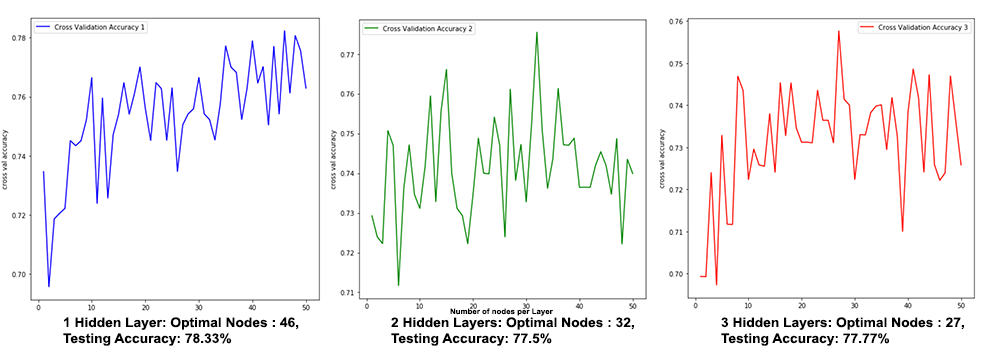
\includegraphics[scale = .50]{graph}
\caption{Output of predictive accuracy for 1,2 and 3 layer ANN's} 
\end{figure}

\subsection{Software Testing: Genetic Program}
Whilst developing each class and the functions associated with the classes, I originally generated a very small set of static data with classifications, with an optimal function that could be used to verify whether the GP was learning or not. 
The first class that was created was GenMember, to create valid random mathematical functions, select parents and update the population. Unfortunately, as it was very difficult to test whether \textit{generate\textunderscore expression} was working, I had to manually verify that this function was producing valid mathematical functions, with complete bracketing in the correct places. To ensure that the \textit{get\textunderscore valid\textunderscore expression} worked, since the generated expression needed to contain all five variables X1,...,X5, the only way that this condition could be checked was to call the function multiple times based on the generation created originally. Using these outputs, which I able to acknowledge that they were correct, I created a small population of 6 individuals. Based on the fitness values given to each of the individuals in the population, I could perform Unit testing on functions such as \textit{tournament\textunderscore selection}, as I knew the sample population. For this function, I could use white box testing within the unit test, to ensure that out of these 6 individuals, 4 were candidates and the best individuals were assigned to be parents. This was tested multiple times to ensure that the best candidates were always being selected. 
 
The next class to test was \textit{ToPrefixParser}. To enable the infix to prefix conversion to be successful, the state of the infix function had to be changed into an acceptable format for 
\textit{get\textunderscore prefix\textunderscore notation} to accept. As this code was used from another source, to initially test this on sample problems, I wrote out infix functions and manually converted them to prefix notation. Using this, I used black box testing to check whether the infix notation being inserted was correctly being converted to prefix notation, on small and larger expressions, to ensure that every expression was being correctly converted. 

Using two expressions that were converted into prefix, I was then able to start testing the \textit{Tree} class. For \textit{make\textunderscore tree}, I used a simple prefix expression
and manually constructed what the tree should look like. If the expected tree followed the same structure as the manually drawn tree, i.e. nodes placed in the correct place, and correct associations with their respective parents, then the \textit{make\textunderscore tree} function was functioning correctly.  This same process was repeated for larger, more complex prefix expressions, to ensure that this function could build any tree, based on any variety of prefix expression.  

To ensure that \textit{find\textunderscore subtree} was performing as it should, rather than trying to find a random nodeID, I chose a specific node to find, such that I was able to perform the search manually and in a 'verbose' mode, such that as the function was running, I could confirm that at every stage, it was reaching the expected node it was meant to.

Another crucial function that needed testing was \textit{swap\textunderscore nodes}. To test this, I used two prefix expressions which simulated parents in their binary tree structures. By inserting and printing the parents that would be crossed over, it was obvious to see that the nodes had been changed before and after the crossover took place. To ensure that this was correct, white box testing was performed to determine that the new children produced were contained in the right variables and contained the correct node values. This was relatively straightforward to test as I could print the new trees produced and compare the original parents to the children, based on the child nodes that I had selected to be crossed over.  This same process was performed for the \textit{mutate\textunderscore node} function, as they both required the tree inputs, and the node(s) to be manipulated, therefore since I selected a specific node to be mutated, I was able to see exactly what it was mutated to, to ensure that this function was performing as expected.\\

The next class that needed testing was the \textit{ToInfixParser} class. To test this class, using a simple problem to begin with, I used a prefix notation expression, and manually converted this to infix notation. Using this as the desired output, I could use black box testing to determine if that prefix expression was converted to the same infix expression in the\textit{conv\textunderscore inf}  function . This was repeated multiple times on small and then bigger problems. To ensure that this was correct, I had to evaluate the newly created infix expressions to ensure that due to the encapsulation of the sub expressions, the numerical output remained the same. If they did, then this test was successful. 

After the children were evaluated, I used white box testing to confirm that the children were in the correct string format to be accepted back into the population. Through this white box testing, I was able to see where the children were checked against the worst members of the population, and then see which members of the population were changed, and to see whether the population sized definitely stayed the same. If the worst members of the population were removed, then this confirmed that the model was starting to learn as it was filtering out worse members of the population. 

Finally, the last section to test was the termination criteria. using a sample population, I was able to track the progress of the population through a few iterations, and kept the termination criteria very flexible, to check that if certain conditions were met, the program would terminate successfully with the correct function being returned as part of the output. 

\subsection{Running the Genetic Program - Training and Testing datasets}
Similar to the ANN, in GPs, it is very common for the network to train using one dataset and to test the predictive classification accuracy on another dataset. During the development of the project, after simple problems were able to produce the correct results, I used a random selection of 10 rows of data from the original dataset which could be used to train the network as a sample, as a validation method to see if the accuracy of training prediction increased over time. If after \textit{n} iterations, the optimal solution was found for example with 90\% training accuracy, this confirmed that the model was learning the data over time, to produce an optimal function. Using this confirmation, I was then able to feed in the full dataset to see if the model would still learn. \\
My first method of testing was to train the GP using the full given data set. After this was done, since another dataset was unavailable, I used the same dataset to test the predictive accuracy of the genetic program optimal equations. Even thought it was thought that this would in theory achieve 100\% predictive accuracy, the GP produced between 70-75\% accuracy. The reason for this is every time a new population is generated, a different area of the search space is explored, which means the function, albeit have the same training and testing data, it will not produce 100\% testing predictive accuracy. 

To make the the ANN and GP more comparable, I also attempted to use the train test split function to split the data into two sets, using 80\% of the data to train the model and 20\% to test the model. The outputs of this can be seen in Figure below [insert graphs of GP and ANN when using TTS]. 

Although K-Fold Cross Validation can be used for the GP by being able to produce the average predictive accuracy of the model, the aim of the project was to find an optimal function that could be used to predict CB. However it is not possible to average multiple expressions which would produce a solution that is equivalent to the predictive classification accuracy produced by K-Fold. Therefore I decided not to use this method as a form of training and testing the datasets. 

\subsection{Genetic Program Experiments}
As an optimal function was being found for smaller problems, I used the actual dataset and altered the parameters to see if the predictive accuracy would increase on more complex problems. To make this process easier, the \textit{train\textunderscore gp} function contained all the parameters that could be optimised, which could affect the predictive accuracy of the model. For every test that was conducted, each test ran for a minimum of \
50 times to ensure that each of the tests were giving consistent results, and to identify any patterns and anomalies that may exist when running various tests.   \\

The first parameter that was changed when testing on the hold out data set was the threshold value to classify a company as 1 or 0. The values of this ranged between 0.1 - 0.9, to see the different classification accuracies when being used on the hold out set.Through the use of box and whisker plots, it was noted that the worst predictive accuracies came from threshold values that were closer to the the values or 0 or 1. When using threshold values of 0.1- 0.4, although the accuracies did improve, there was a significant overlap between all the accuracies. Not just this, but as Figure (?) shows they also had a very high variance and standard deviation. Because of this, they were considered to be too volatile to give a consistently accurate predictive classificiation accuracy. 
\begin{figure}[h]
\centering
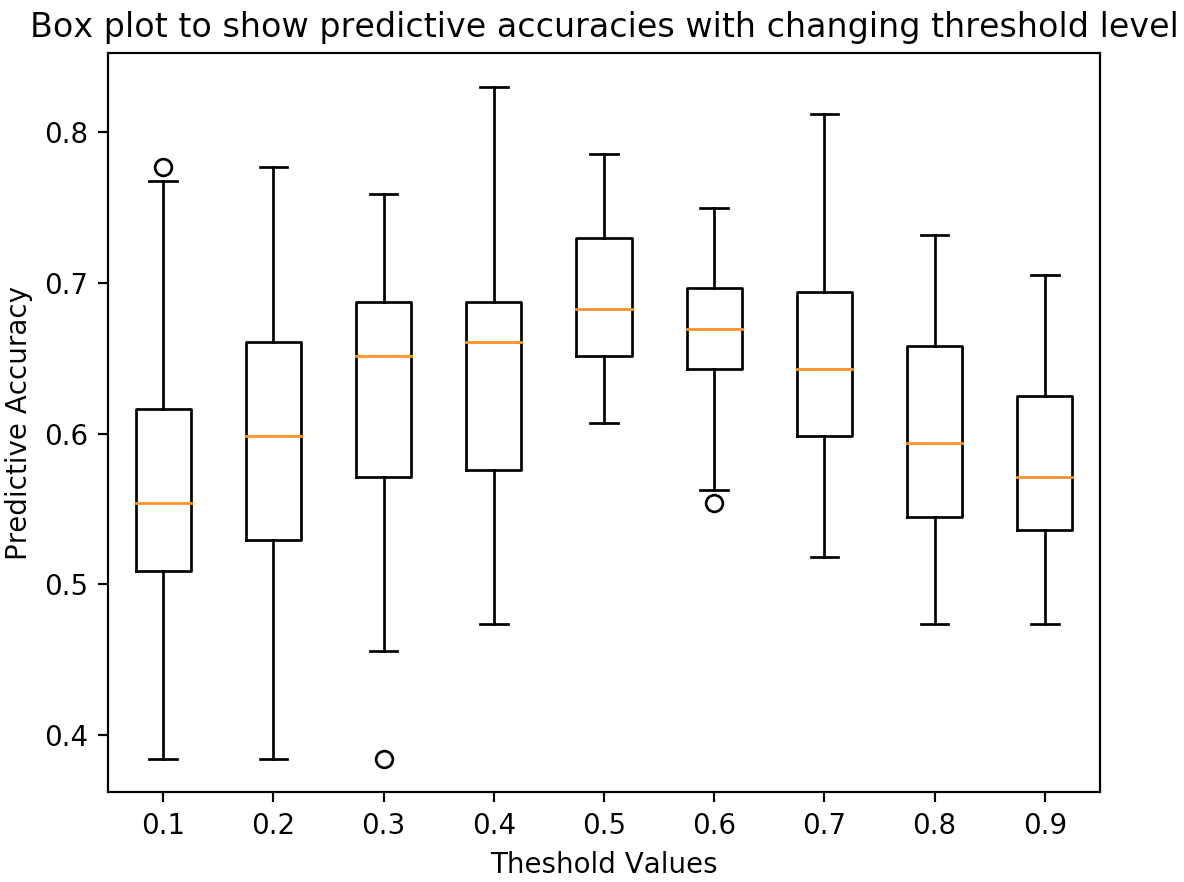
\includegraphics[scale = .30]{thresh}
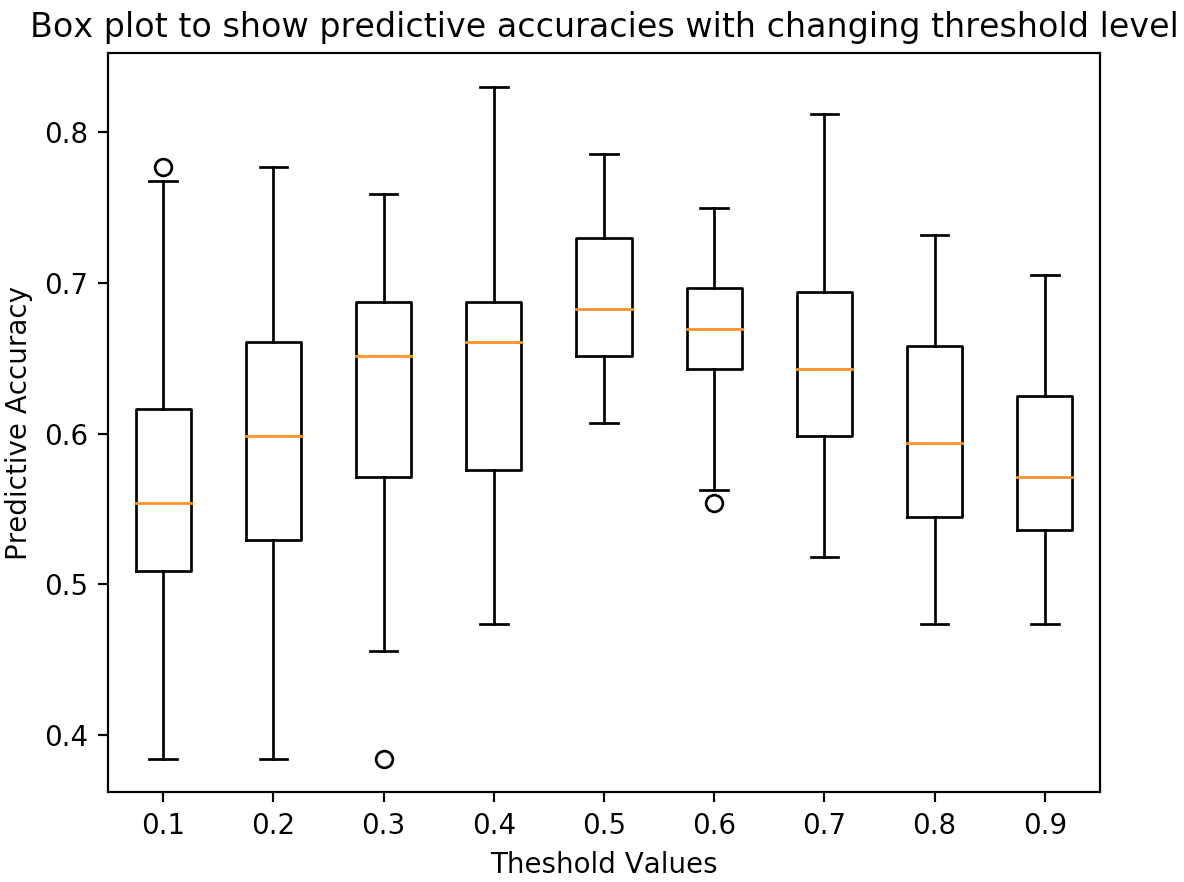
\includegraphics[scale = .30]{thresh} 
\caption{Output of predictive accuracy for 1,2 and 3 layer ANN's} 
\end{figure}


The next test that was performed was using different selection methods. As the selection function is also a parameter, this increased the flexibility of the model, as I was able to create another selection mechanism, select best to train and test the model. This selection function selected the best two individuals in the population every single time. The expectation of this is that when training the model, it would plateau off as the fitness values would start to converge to a fitness value similar to the parents, therefore converging at a local optimal solution. This did occur as can be seen in figure(?) which compares the fitness errors of using tournament selection against select best. [insert figure here].

Another parameter that could be tuned was the maximum number of iterations allowed before the model terminates. This involved using a variety of different max iteration values, to see if this made any difference to the predictive accuracies. In theory, if there were too few iterations, then the model would not be able to learn sufficiently. If there were too many iterations, then there is a possibility that learning would eventually stop, and that this would be very computationally expensive to try to find an optimal solution to this problem. The results of this can be seen in Figure (?) where when using 10 and 100 as the parameter values, the graph clearly indicated that learning was still occurring, however, after when the maximum iterations were 1000, 2000, 3000 , they showed signs of convergence, and eventually stopped learning as quickly. [insert figure here]. However, when using over 1000 members in the population, this showed signs of poor predictive  accuracy.



%varying parameters - much more flexible. 
%changing the cuttoff point 
%limits  cause SO error
%selection methods



\subsection{evaluation of ANN and GP }
%talk about performance of each of them
% talk about accuracy of them
% talk about what is better and why
 

\newpage
\section{Comparisons of Artificial Neural Networks and Genetic Programs}
\newpage
\section{Critical assessment of the project }
\subsection{What was Successful}

\newpage
\section{Future Work}
\subsection{Possible Improvements}

\newpage
\section{Conclusion}

\end{document}




